%% This is an example first chapter.  You should put chapter/appendix that you
%% write into a separate file, and add a line \include{yourfilename} to
%% main.tex, where `yourfilename.tex' is the name of the chapter/appendix file.
%% You can process specific files by typing their names in at the 
%% \files=
%% prompt when you run the file main.tex through LaTeX.

\begingroup%
\makeatletter%
\cleardoublepage%
\let\newpage\relax%
\let\clearpage\relax%
\vspace*{\fill}%
\vspace*{\dimexpr-50\p@-\baselineskip}% Remove the initial
%% -default- 50pt gap (plus 1 line) 
\chapter{A New, Autonomous Device Captures \emph{In Situ} Variation in Oxygen Consumption and Community Metabolism at Very Fine Time Scales}
\label{AppA}
\let\thefootnote\relax\footnote{{\setlength{\parindent}{0pt}In preparation as:\\\\Collins, J. R., P. D. Fucile, G. McDonald, J. E. Ossolinski, R. G. Keil, J. R. Valdes, S. C. Doney, and B. A. S. Van Mooy. A new, autonomous device captures \emph{in situ} variation in oxygen consumption and community metabolism at very fine time scales.}}
\vspace*{\fill}%
\endgroup%

\clearpage
\section{Abstract}
We describe a new, incubation-based instrument that is deployed \emph{in situ} to determine rates of respiration and primary production in a wide range of marine and aquatic ecosystems. During deployments at a coastal pier and in the open ocean, the PHORCYS (\emph{PHO}tosynthesis, \emph{R}espiration, and \emph{C}arbon-balance \emph{Y}ielding \emph{S}ystem) captured large natural fluctuations in oxygen consumption and production rates over hourly timescales that were missed by traditional methods. The instrument, which uses fluorescence-quenching optodes fitted into separate light and dark chambers, yielded metabolic rate estimates that generally agreed with (1) two-point Winkler titrations and (2) a series of shipboard incubations. Piston-like magnetically coupled actuators are used to open and close the PHORCYS chambers, allowing the instrument to take in and discharge multiple samples (and make multiple rate estimates) in the course of each deployment. We also present a new method for estimating uncertainties in metabolic rates calculated from continuous dissolved oxygen data. The method, which is based on a common approach to time-series analysis in physical oceanography, provides investigators with an alternative to the standard error of the regression slope in instances when true replication cannot be achieved. Multiple successful, unattended deployments of the PHORCYS in the open ocean represent a step toward long-term, fully autonomous observations of community metabolism.
\clearpage
\section{Introduction}
Accurate, reproducible, and cost-effective estimates of aerobic respiration and primary production are essential for research across a diverse array of disciplines in the environmental sciences (del Giorgio and le B. Williams, 2005; Staehr et al., 2012; Volkmar and Dahlgren, 2006). Rate measurements of these two metabolic parameters can be applied to various problems, including validating the biogeochemical components of global climate models (Denman et al., 2007), determining the trophic status of surface-water planktonic communities in open ocean ecosystems (le B. Williams, 1998), measuring rates of biological oxygen demand (BOD) in treated wastewater (Spanjers et al., 1994), and identifying unexpected metabolisms in the deep ocean (Reinthaler et al., 2010).

While an increasing demand for metabolic rate data has encouraged the development of many different methods for estimating rates of photosynthesis (Ducklow and Doney, 2013), the number of new methods for measuring aerobic respiration at the community scale has lagged behind considerably (del Giorgio and le B. Williams, 2005). The majority of field-based methods for measuring rates of respiration and primary production in the ocean fall largely into two categories: (1) \emph{in situ} geochemical tracer techniques that track changes in dissolved oxygen and carbon dioxide within ocean water masses (e.g., the surface mixed layer), and (2) \emph{in vitro} incubation techniques that track the rates at which plankton exchange oxygen or carbon dioxide in discrete seawater samples (i.e., bottle incubations). The merits and faults of these two categories of approaches have been vigorously debated (Duarte et al., 2013; Ducklow and Doney, 2013; le B. Williams et al., 2013). The former category has benefited considerably from recent advances in sensor technology (Moore et al., 2009). By maximizing the extent to which sensors are integrated into the surrounding environment, low-power instruments increase the spatial and temporal resolution of geochemical tracers \emph{in situ} and permit increasingly autonomous, long-term deployments (Porter et al., 2009; Prien, 2007; Riser and Johnson, 2008).

By contrast, sensor development has spurred relatively few technical advances in \emph{in vitro} incubation techniques. The traditional two-point light and dark bottle incubation technique (Gaarder and Gran, 1927) and the \textsuperscript{14}C incubation method (Steeman Nielsen, 1952) continue to dominate incubation-based studies, although a number of other methods have been introduced in recent decades (Bender et al., 1987; Kenner and Ahmed, 1975; Robinson and le B. Williams, 2005). These traditional methods may be prone to error from (1) contamination, disruption, or bias introduced through the process of obtaining seawater samples and preparing them for incubation (Suter et al., 2016); (2) unrepresentative incubation conditions that do not faithfully reproduce the variations in temperature and light inherent in natural systems; and (3) so-called ``bottle effects'' associated with low-volume incubations which may limit nutrient availability (Furnas, 2002) or induce unnatural changes in community structure (Calvo-Díaz et al., 2011; Venrick et al., 1977); and (4) the lack of temporal resolution inherent in measurements based only on two endpoints. In any study where incubations are used, the choice of incubation methodology places inherent limits on the spatial and temporal resolution of the data collected (Karl et al., 2001).

We describe here the \emph{PHO}tosynthesis, \emph{R}espiration, and \emph{C}arbon-balance \emph{Y}ielding \emph{S}ystem (PHORCYS), a high volume, light and dark chamber incubation system for obtaining rates of primary production and respiration at high temporal resolution under \emph{in situ} conditions. In designing the instrument, we endeavored to minimize the four major sources of uncertainty associated with traditional incubation-based methods while constructing a system that functions autonomously. We describe two versions of the instrument (``A'' and ``B,'' respectively) in which different mechanisms were used to effect closure of the incubation chambers. In both cases, we sought to eliminate or reduce the need for repeated wet-chemical measurements in the field (e.g., Winkler oxygen titrations). We first describe design and validation of the PHORCYS using two independent methods, and then present results of several deployments of the instrument in different ecosystem types.
\section{Materials and Methods}
\subsection{Instrument Design and Operation}
Both the ``A'' and ``B'' model PHORCYS systems are composed of only a few basic components, making the designs highly scalable and cost-effective (\autoref{fig:aan1}a,b). In nearly all instances, ``off the shelf'' components of different size or capacity can be easily substituted for those we describe here.
\subsubsection{``A'' Model}
\begin{figure}[!b]
\centering
\includegraphics[width=1\textwidth]{Fig_A-1.pdf}
\captionsetup{font={footnotesize}}
\caption[Design and deployment of the PHORCYS]{Design and deployment of the PHORCYS. Major components of the ``A'' and ``B'' model PHORCYS instruments are illustrated in (a) and (b), respectively. The current, ``B'' model device uses magnetically-coupled actuators, allowing for multiple openings and closings of the chambers during a single deployment. The ``B'' model instrument also includes several sensors for collection of auxiliary data, including photosynthetically active radiation (PAR), conductivity, ambient temperature, transmissivity, and chlorophyll fluorescence. The ``B'' model also includes a third optode to measure dissolved oxygen concentrations in the ambient water mass outside of the two chambers. (c) Rigging scheme for open-ocean deployments from a drifting surface mooring, as described in the text.
}
\label{fig:aan1}
\end{figure}
For construction of the prototype ``A'' model instrument (\autoref{fig:aan1}a), two 2.5 L Niskin-style sampling bottles (opaque polyvinylchloride and transparent polycarbonate plastic, respectively; actual usable volume, 2.6 L; General Oceanics, Inc., Miami, FL, USA) and a watertight power supply, control, and data recording module were mounted to an aluminum frame. (In experiments, the polycarbonate plastic reduced photosynthetically active radiation (PAR) within the transparent chamber to 83\% of incident strength.) Into each Niskin bottle incubation chamber a fast-response, fluorescence quenching oxygen optode (Aanderaa model 4330F; accuracy \textless{} 8 $\mu$M O\textsubscript{2}; resolution \textless{} 1 $\mu$M O\textsubscript{2}; Aanderaa Data Instruments, Inc., Bergen, Norway) was mounted using a watertight flange assembly. Each flange assembly accommodated a spring-loaded mechanism that held the bottle endcaps open during deployment and then closed them to initiate the incubation once the instrument was in place. Closure of the chambers for incubation was effected using a time-release ``burn wire'' system. Each watertight flange assembly accommodated a fusible burn wire plug to which the bottle end caps were rigged prior to each deployment. When a sufficient current was applied to the burn wire, the wire corroded and allowed the bottle endcaps to close; the chambers were then sealed and the incubation began. This design allowed us to conduct a single incubation during each deployment after settings had been uploaded to the instrument via a serial cable. In the ``A'' model deployments (\autoref{fig:aan2}, 
\includegraphics[height=\fontcharht\font`\B]{images/Fig_A-Inline1.pdf} symbols), we programmed the chambers to close approximately 45 minutes after the PHORCYS had reached the desired depth.
\subsubsection{``B'' Model}
Following our initial deployments in 2012 with the ``A'' model instrument, we redesigned the chamber closure system to accommodate multiple incubations in the course of each deployment. In addition, the ``B'' model instrument (\autoref{fig:aan1}b) includes several sensors for collection of auxiliary environmental data. The data from these sensors (a third external optode to monitor dissolved oxygen concentrations in the water mass outside of the two chambers, photosynthetically active radiation, light transmission, chlorophyll fluorescence, temperature, and conductivity) may be used to enhance the investigator's interpretation of dissolved oxygen fluxes within the chambers. In the ``B'' model instrument, both chambers (usable vol. 5.7 L) are constructed of the same non-reactive polycarbonate plastic; the opaque chamber was darkened by application of a coating to the outside of the cylinder. All of the components are mounted to a load-rated stainless steel frame, allowing the instrument to operate to a depth of 100 m. The ``B'' model chambers are opened and closed for incubation by a magnetically coupled actuator commanded by the control electronics. The seals are tapered to avoid the use of rubber O-rings that might have introduced a source of organic contamination into the sample water. A single pressure case holds the controller/data logger electronics and power source. The ``B'' model instrument uses three Aanderaa model 4531D optodes, which offer accuracy and resolution similar to the 4330F model optodes but use significantly more robust bulkhead connectors.
\begin{SCfigure}[0.5][!t]
\centering
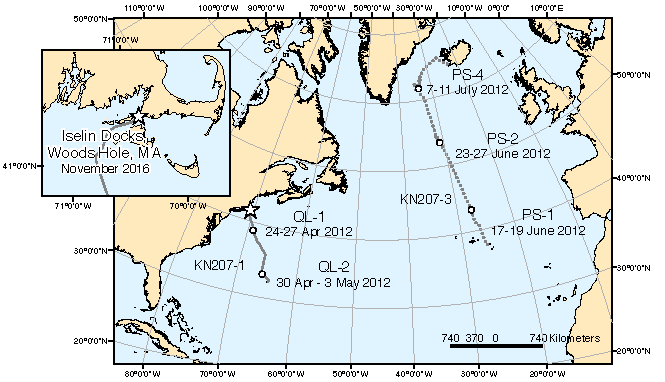
\includegraphics[width=0.7\textwidth]{Fig_A-2.pdf}
\captionsetup{font={footnotesize}}
\caption[Locations of PHORCYS deployments described in the text]{Locations of PHORCYS deployments described in the text. Primary map: Unattended open-ocean deployments from a surface mooring were conducted using the PHORCYS Model ``A'' at 5 stations during two cruises aboard the \emph{R/V Knorr}. Stations QL-2 and QL-2 were conducted during cruise KN207-1; PS-1, PS-2, and PS-3 were conducted during cruise KN207-3. Inset: Pierside deployments using the PHORCYS Model ``B'' were conducted in November 2016 at the Iselin Marine Facility in Woods Hole, MA, USA.}
\label{fig:aan2}
\end{SCfigure}

Depending on data rates, the nominal sampling power consumption is 50 mA at 12V, while standby current is 2 mA. This allows a single battery pack to operate the instrument for up to 30 days in unattended deployment mode. Data are recorded in an ASCII fixed-field format onto a micro SD card in a DOS readable format. For attended deployments, a combination communications and external power port provides the ability to observe data in real time, allow program updates, download data, and power the instrument indefinitely. The sampling interval is nominally set to one minute, though data can be collected as frequently as every 15 s. The ``B'' model acquisition program determines sampling activity by way of a real-time clock. The chambers can thus be programmed to open at any time, allowing the investigator to make multiple incubations of any desired length. In the configuration used to acquire the data presented here, (\autoref{fig:aan2}, 
\includegraphics[height=\fontcharht\font`\B]{images/Fig_A-Inline2.pdf} symbol) the chambers were programmed to open at or around sunrise and the same operation was repeated at sunset, providing two incubations in each 24-hour period that aligned with the beginning and end of the photoperiod. The chambers are opened and then closed sequentially (i.e., one after the other) to reduce total current draw from the power source. The chambers remain open for 30 minutes at the outset of each incubation, providing sufficient time for the water to be fully exchanged before the chamber then closes; we confirmed this flushing time was sufficient in both quiescent and flowing (\textasciitilde{} 1 m s\textsuperscript{-1}) waters using a series of tests with a tracer dye (results not shown).
\subsection{Instrument Deployments}
We conducted 6 deployments of the PHORCYS in 3 distinct ecosystem types in the North Atlantic basin (\autoref{fig:aan2}; \autoref{table:aan1} and \autoref{table:aan4}). Open-ocean deployments of the ``A'' model instrument were conducted during cruises aboard the R/V \emph{Knorr}; during these deployments, the instrument was suspended at various depths in the euphotic zone from an unattended, drifting surface buoy (\autoref{fig:aan1}c). Deployment and recovery were accomplished in 45-60 minutes from a standard oceanographic research platform (\autoref{fig:aan5}). Pierside deployments were conducted at the Iselin Marine Facility, Woods Hole, MA, USA (41$^{\circ}$ $31'24''$ N 70$^{\circ}$ $40'20''$ W); the site adjoins a highly productive coastal embayment. The open-ocean deployments (2 to 7 days in length) were made in ``quasi-Lagrangian mode,'' with the goal of tracking a single water mass for the duration of the deployment. Oxygen concentrations ($\mu$mol L\textsuperscript{-1} O\textsubscript{2}), percent saturation, and temperature were then recorded for each chamber at one-minute intervals. Both the coastal (``B'' model) and open-ocean (``A'' model) data were corrected for salinity upon recovery using concurrent \emph{in situ} salinity observations and manufacturer-supplied correction coefficients.
\begin{SCfigure}[0.5][!t]
\centering
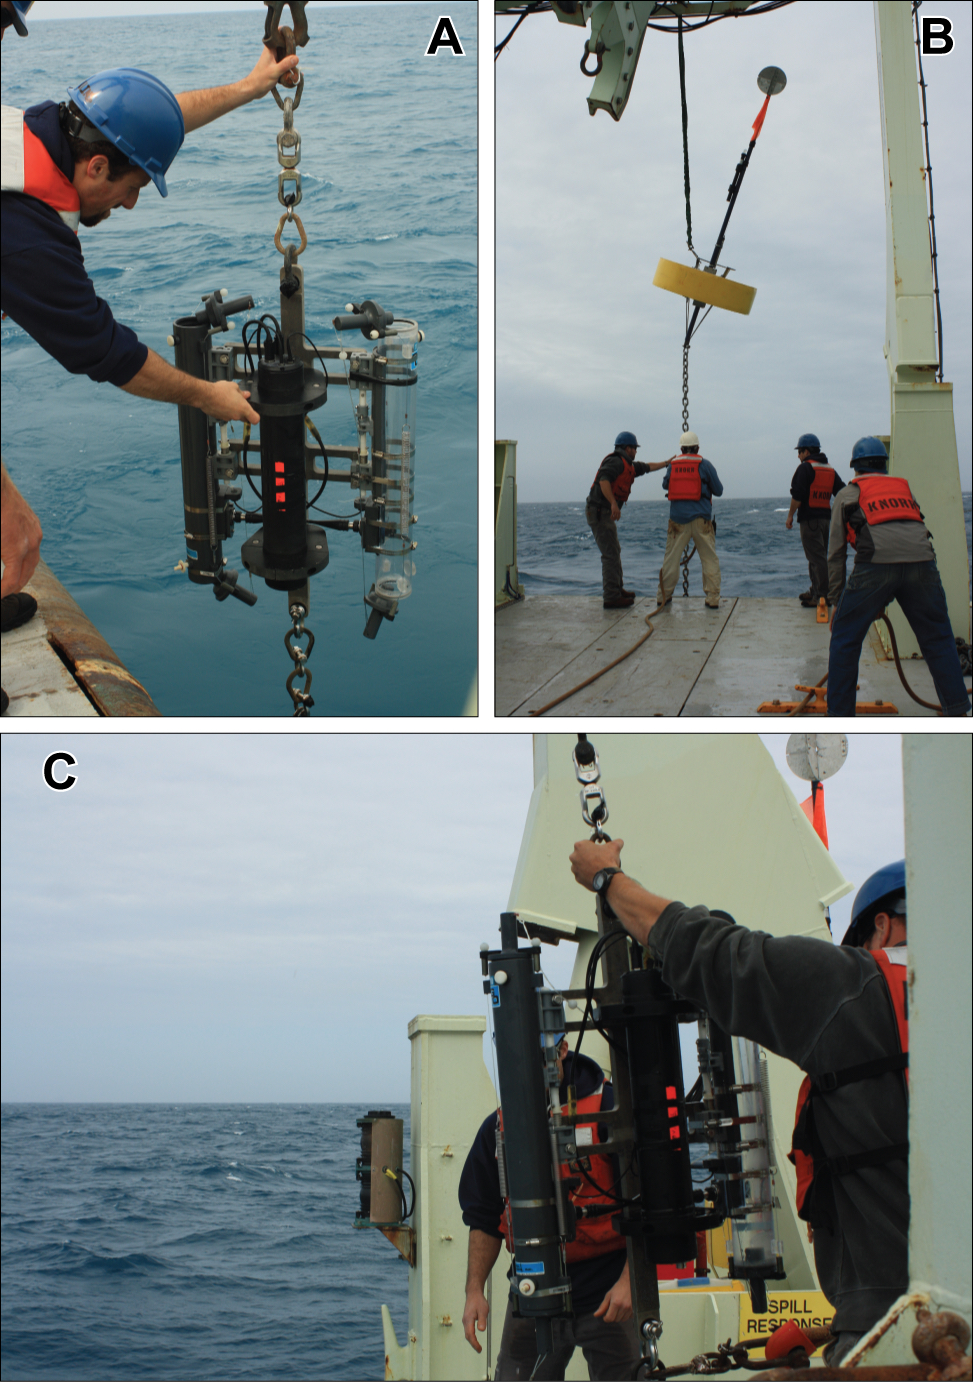
\includegraphics[width=0.6\textwidth]{Fig_A-S1.jpg}
\captionsetup{font={footnotesize}}
\caption[Deployment and recovery of the PHORCYS ``A'' model from a drifting surface mooring during June 2012]{Deployment and recovery of the PHORCYS ``A'' model from a drifting surface mooring during June 2012. Prior to each deployment, a text interface was used to set mission parameters via a serial cable and personal computer. Using the plain-language interface, one can calibrate the optodes, specify the ``burn time'' at which the chambers should close, and adjust the sampling interval. (a) Both PHORCYS chambers are cocked open using a burn wire assembly immediately prior to initial deployment. (b) The surface mooring is recovered. (c) The PHORCYS is recovered with both chambers sealed.}
\label{fig:aan5}
\end{SCfigure}
\subsection{Instrument Calibration and Choice of Deployment Depth}
Optodes were calibrated before each pierside deployment and prior to each research cruise using a two-point method. An air-saturated solution was obtained by bubbling ambient air for approx. 30 minutes through a sufficient volume of Milli-Q water using an aquarium stone; a zero oxygen solution was obtained by dissolving an excess of reagent-grade Na\textsubscript{2}SO\textsubscript{3} into a beaker containing Milli-Q water. The optodes were then calibrated at atmospheric temperature and pressure, as recommended by the manufacturer. At the open-ocean stations (Model ``A'' instrument), the PHORCYS deployment depth was chosen based on profiles of PAR from shipboard hydrocasts. Pierside deployments of the ``B'' model instrument were conducted at a depth of 1.5 m.
\subsection{Instrument Validation by Two Independent Methods}
First, to validate the optodes' ability to accurately track respiration, we used a standard analytical method --- two-point Winkler titration --- to determine dissolved oxygen consumption in triplicate water samples at the beginning and end of each deployment (for ``A'' model data) or incubation period (for ``B'' model data). Winkler titrations were conducted in 125 mL BOD bottles according to EPA Method 360.2 as modified for shipboard determination in seawater (Knapp et al., 1989). Initial Winkler titrations were made in samples collected within 15 minutes of deployment using a Niskin or Go-Flo bottle suspended at the same depth as the instrument. A set of three darkened 125 mL BOD bottles containing water from the same Niskin or Go-Flo bottle was incubated at \emph{in situ} temperature until the PHORCYS was recovered (``A'' model instrument) or the incubation period ended (``B'' model instrument); these samples were then sacrificed according to the same protocol. The BOD bottles used in these incubations were triple-rinsed with 10 \% HCl and then Milli-Q water prior to sampling. All reagents for Winkler titrations were A.C.S. grade or better; the Na\textsubscript{2}S\textsubscript{2}O\textsubscript{3} titrant was standardized daily. Amperometric titration was performed using an autotitrator (Metrohm 904 Titrando; Metrohm USA, Inc., Riverview, FL).

As an additional means of comparison during the ``A'' model (open ocean) deployments, we also tracked changes in dissolved oxygen in a series of continuously monitored shipboard bottle incubations. Water from the PHORCYS deployment depth was retrieved for these incubations from a hydrocast made within one hour of deployment. Incubations were conducted with gas-tight, 300 mL glass bottles, which had been soaked prior to deployment for \textgreater{} 2 months in Milli-Q water. At least 5 replicates were used for each series of measurements. Determination of dissolved oxygen was made at 3- to 9-hour intervals using optode spot minisensors (PreSens PSt3; Precision Sensing GmbH, Regensburg, Germany; Warkentin et al., 2007) that were glued to the inside surfaces of the bottles using food-quality silicone cement. The use of these optode spots eliminated the need for drawing of aliquots from the sample bottles. The incubations were conducted in the dark at \emph{in situ} temperature as described in Edwards et al. (2011).
\subsection{Data Analysis}
\subsubsection{PHORCYS Rate Calculations}
Volumetric rates of gross community respiration (GR) and net community production (NCP) were calculated by linear least-squares regression of observations of dissolved oxygen concentration over the length of the deployment (``A'' model data) or incubation period (``B'' model data). We assumed the only significant chemical reactions contributing to oxygen consumption and evolution in the two chambers were aerobic respiration and photosynthesis. These redox reactions can be represented as
\begin{equation} \label{eq:aan1}
{{\text{C}}_{\text{6}}}{{\text{H}}_{{\text{12}}}}{{\text{O}}_{\text{6}}} + {\text{ 6}}{{\text{O}}_{\text{2}}} \to {\text{6C}}{{\text{O}}_{\text{2}}} + {\text{ 6}}{{\text{H}}_{\text{2}}}{\text{O}}
\end{equation}
and
\begin{equation} \label{eq:aan2}
{\text{6C}}{{\text{O}}_{\text{2}}} + {\text{ 6}}{{\text{H}}_{\text{2}}}{\text{O }} + h\nu  \to {{\text{C}}_{\text{6}}}{{\text{H}}_{{\text{12}}}}{{\text{O}}_{\text{6}}} + {\text{ 6}}{{\text{O}}_{\text{2}}}
\end{equation}
As is the case with the classic light and dark bottle incubation technique, we assumed that only respiration was taking place in the dark (i.e., GR; reported as positive quantities), while both reactions were taking place simultaneously in the presence of light (i.e. NCP). Finally, where possible, we calculated estimates of gross primary productivity (GPP) according to the relationship
\begin{equation} \label{eq:aan3}
{\text{GPP }} = {\text{ NCP }} + {\text{ GR}}
\end{equation}
\subsubsection{Rate Calculations from Winkler Titration Samples and Sensor Spot Incubations}
For the Winkler titration samples, oxygen consumption rates were calculated using a simple difference of means (mean of concentrations in samples sacrificed at final timepoint $-$ mean of concentrations measured in initial sample). For the sensor spot incubations, we calculated rates for each bottle using a linear least-squares regression of all observations recorded over the time period; we then averaged the rates obtained for the various replicates to obtain a final estimate.
\subsubsection{Calculation of Uncertainties in Metabolic Rate Estimates}
\label{ssec:Calculation of Uncertainties in Metabolic Rate Estimates}		
Uncertainties in rates based on the Winkler titration method were determined from the standard deviations of the dissolved oxygen concentrations measured in the replicates at each timepoint. For rates based on the sensor spot incubations, we used the standard error of regression. To estimate the uncertainties in our PHORCYS rate estimates, we adapted a technique traditionally applied to time-series data in physical oceanography (Emery and Thomson, 2001). The ideal means of estimating uncertainties in PHORCYS rates would have been true biological replication, i.e., the simultaneous deployment of several identical instruments in the same water mass. One could then have used the standard deviation of the rate measurements in each different instrument~as an estimate of the overall uncertainty. Because we had only one instrument --- an exceedingly common situation in oceanographic work --- such true replication was not possible. The standard error of the regression slope provides one possible estimate of uncertainty in time-series dissolved oxygen data; for example, this common approach was recently applied to data from \emph{in situ} chamber incubations of sinking marine particle material (McDonnell et al., 2015). However, we assumed that the standard error of regression would significantly underestimate the true uncertainty in our estimates since it does take into account the reduced number of degrees of freedom in such a time series. Because the data points in such a dissolved oxygen time series are not independent of one another, there are almost always far fewer effective degrees of freedom $N^*$ in such data than the number of observations (i.e., data points) \emph{N} (Emery and Thomson, 2001).

Our approach was the following: For each time series of dissolved oxygen concentrations, we first approximated the integral time scale \emph{T} of the data according to
\begin{equation} \label{eq:aan4}
T = \frac{1}{{C(0)}}\int\limits_0^{{B_0}} {C(\tau )d\tau }
\end{equation}
where \emph{C}(0) is the value of the autocorrelation function \emph{C} of the time series at lag $\tau$ = 0, and \emph{B}\textsubscript{0} is the value of the autocorrelation function at the first zero crossing, which (after, e.g., Talley et al., 2011) we use as an estimate of the timescale of decorrelation. We then followed the method of Emery and Thompson (Emery and Thomson, 2001) to estimate the effective number of degrees of freedom $N^*$ from \emph{T}, \emph{N}, and $\Delta$\emph{t}, where $\Delta$\emph{t} is the sampling interval of the data
\begin{equation} \label{eq:aan5}
N^* = \frac{{N\Delta t}}{T}
\end{equation}
In this formulation, $\Delta$\emph{t} is therefore the total length of the oxygen time series in which the rate estimate was made. Finally, we used this $N^*$ to obtain ${s_{{{\hat \beta }_{1,adj}}}}$, an adjusted estimate of the standardized uncertainty in the slope parameter of the regression (i.e., ${\hat \beta _1}$, the rate of dissolved oxygen consumption or production), according to
\begin{equation} \label{eq:aan6}
{s_{{{\hat \beta }_{1,adj}}}} = \sqrt {\frac{{SSE}}{{N^* - 2}}\frac{N}{\Delta }}
\end{equation}
where \emph{SSE} is the sum of the squared errors from the fit of the regression, i.e., $\sum\limits_{i = 1}^N {{{({y_i} - {{\hat y}_i})}^2}}$, \emph{N} is the number of observations (as above), and $\Delta$ is the determinant $N{S_{xx}} - S_x^2$. Those familiar with least-squares regression will observe that \autoref{eq:aan6} is simply the formula for calculation of the standard error of the regression slope in the unweighted case, except that $N^*$ is used instead of \emph{N}. A MATLAB script provided online (see \autoref{sec:Availability of Data and Code}, below) can be used to estimate the $N^*$-based uncertainty in a dissolved oxygen time series from the PHORCYS or any other source.
\section{Results and Discussion}
\subsection{PHORCYS Metabolic Rate Estimates}
We observed a significant degree of daily and hourly variability in the time series data from each PHORCYS deployment (e.g., \autoref{fig:aan3}). This variability manifested itself in a wide range of daily metabolic rate estimates (\autoref{table:aan1} and \autoref{table:aan4}), indicating PHORCYS integrated signals from diverse biological and physical forcings, including cyclical changes in cellular growth cycle, surface-layer water temperature, and irradiance. Daily rates of GR were estimated from dark chamber data for all ``A'' and ``B'' model PHORCYS deployments (\autoref{table:aan1}). Erroneous readings from one of the optodes and a system malfunction prevented us from recovering usable NCP data from the transparent chamber during two of the open-ocean ``A'' model deployments. During the 24-27 April 2012 deployment, the chosen depth of 29 m provided insufficient PAR (\textless{} 3\% of surface intensity) to support photosynthesis in the transparent chamber; we could not calculate NCP or GPP for this station (\autoref{table:aan4}). An obstruction prevented the transparent chamber from closing during the November 2016 ``B'' model deployment, allowing us to recover useful data from only the dark chamber.
\begin{figure}[!t]
\centering
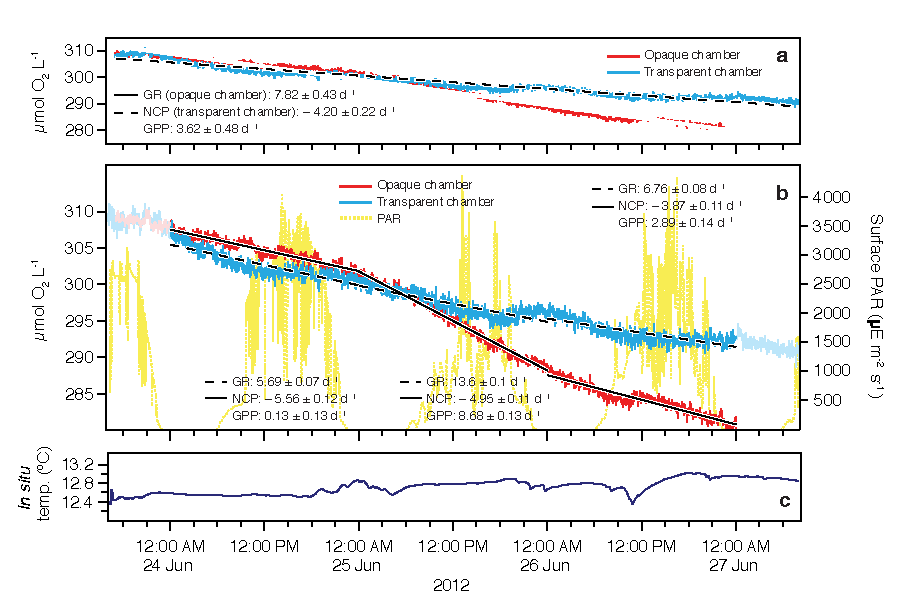
\includegraphics[width=1\textwidth]{Fig_A-3.pdf}
\captionsetup{font={footnotesize}}
\caption[Unattended observations of ecosystem metabolism made with the PHORCYS at a sub-Arctic site]{Unattended observations of ecosystem metabolism made with PHORCYS during a sub-Arctic, open-ocean deployment aboard the R/V \emph{Knorr}. A midsummer bloom of a calcifying phytoplankton species was in progress at the site (Collins et al., 2015) when these observations were made. Estimates (in units of $\mu$mol O\textsubscript{2} L\textsuperscript{-1} d\textsuperscript{-1}) of gross community respiration (GR) and net community production (NCP) were obtained by linear least-squares regression for (a) the entire length of the deployment and (b) for each full, 24-day during the deployment. The various regressions are shown as traces (GR as solid trace; NCP as dashed trace) superimposed over the instrument data. GPP was calculated as the difference between GR and NCP based on \autoref{eq:aan3} in the text. Uncertainties were determined using the effective degrees of freedom method described in \autoref{ssec:Calculation of Uncertainties in Metabolic Rate Estimates} of the text. (c) Diel warming of the surface layer is evident in \emph{in situ} temperature data.
}
\label{fig:aan3}
\end{figure}

We captured daily rates of GR ranging from 1.82 $\pm$ 0.18 $\mu$mol O\textsubscript{2} L\textsuperscript{-1} d\textsuperscript{-1} at a mid-latitude station in the North Atlantic to 10.52 $\pm$ 7.51 and 18.93 $\pm$ 1.87 $\mu$mol O\textsubscript{2} L\textsuperscript{-1} d\textsuperscript{-1} in two different water masses at the Woods Hole pier in early November (\autoref{table:aan1}). The wide variation in GR we observed with the PHORCYS covers a significant range of the rates for marine systems compiled by Robinson and Williams (2005). Daily rates of GPP captured by the PHORCYS ranged from essentially zero on several days at a mid-latitude station in the North Atlantic (\autoref{table:aan4}) to 8.68 $\pm$ 0.13 $\mu$mol O\textsubscript{2} L\textsuperscript{-1} d\textsuperscript{-1} for one 24-hour period at during a coccolithophore bloom (Collins et al., 2015) in the sub-Arctic North Atlantic (\autoref{fig:aan3}). Rates of NCP ranged from -1.98 $\pm$ 0.39 $\mu$mol O\textsubscript{2} L\textsuperscript{-1} d\textsuperscript{-1} to -5.56 $\pm$ 0.12 $\mu$mol O\textsubscript{2} L\textsuperscript{-1} d\textsuperscript{-1} (\autoref{table:aan4}). Increasing evidence suggests the significant sub- and inter-daily variation in metabolic activity captured by the PHORCYS exists in all almost natural aquatic systems (Caffrey, 2004; Collins et al., 2013; Staehr et al., 2012); even in oligotrophic waters, respiration and production rates may change significantly from one day (or hour) to the next, even as the system maintains an overall state of near trophic balance (Aranguren-Gassis et al., 2012). The types of fluctuations we observed in the various dissolved oxygen time series obtained from the PHORCYS appear to be characteristic of incubation-based \emph{in situ} instruments. McDonnell et al. (2015) and Boyd et al. (2015) both observed similar behavior in dissolved oxygen data during recent deployments of an \emph{in situ} device that measures oxygen consumption rates on marine particles.
\subsection{Performance of Method for Estimation of Uncertainties}
Our method of estimating uncertainties in PHORCYS rates produced values of $N^*$ that were typically \textless{}\textless{} \emph{N}, the number of observations in the given dissolved oxygen time series (\autoref{table:aan2}). Using the effective degrees of freedom, we obtained adjusted uncertainty estimates for our PHORCYS rates (${s_{{{\hat \beta }_{1,adj}}}}$) which were much greater in each case than the standard error of the regression slope, ${s_{{{\hat \beta }_{1}}}}$ (compare 24.8 \% and 3.4 \% mean precision, respectively; \autoref{table:aan2}). One disadvantage of estimating uncertainty using $N^*$ is that the uncertainty will be least somewhat proportional to the length of the time series considered. However, the method provides a more honest estimate of error that considers both the precision of the measurements and their number.
\subsection{Evaluation of Instrument Performance Using Independent Methods}
\begin{SCfigure}[0.5][!t]
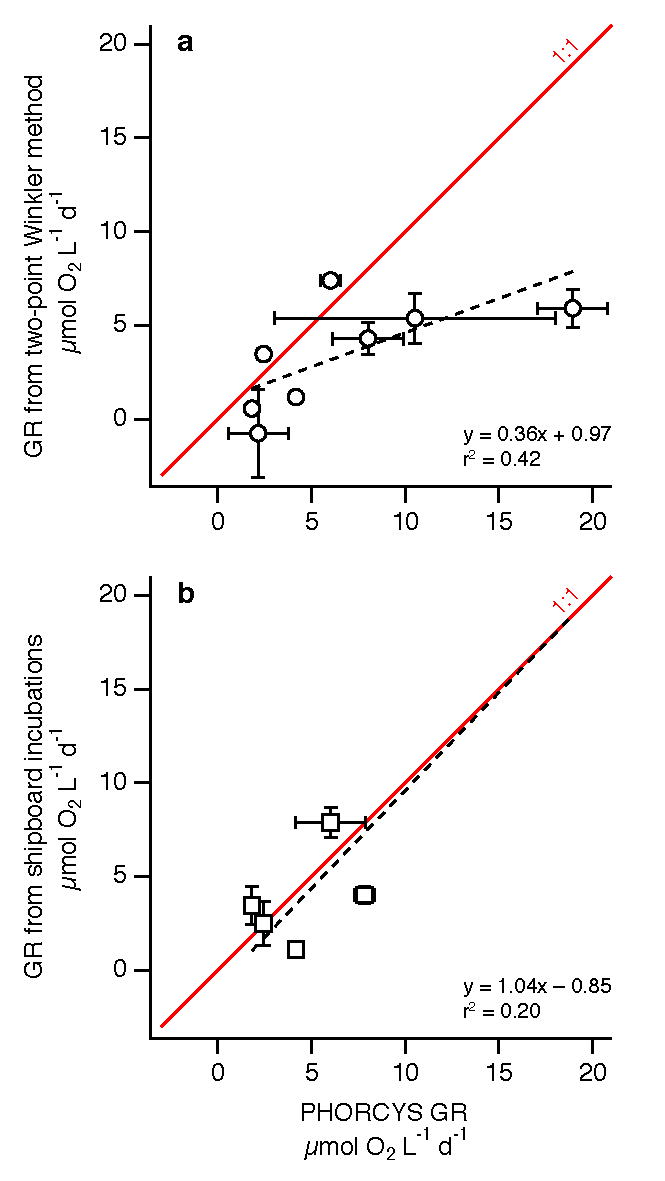
\includegraphics[width=0.5\textwidth]{Fig_A-4.pdf}
\captionsetup{font={footnotesize}}
\caption[Comparison of community respiration rate estimates from the PHORCYS with two other methods]{Comparison of community respiration (GR) rate estimates from the PHORCYS (\emph{x}-axis) with rates determined by (a) the two-point Winkler titration method and (b) a series of shipboard bottle incubations using optode sensor spots. A Type II (major axis) regression was fit to each set of paired observations using the lmodel2 package for R (Legendre, 2014). A red 1:1 line is superimposed in each panel for reference.}
\label{fig:aan4}
\end{SCfigure}
PHORCYS estimates of community respiration were systematically higher than those calculated for the same waters using the two-point Winkler titration method (\autoref{fig:aan4}a; \autoref{table:aan1}). While there was a significant correlation between estimates from the two different methods (r\textsuperscript{2} = 0.42; \emph{p} \textless{} 0.01), the traditional Winkler titration approach appeared to underestimate rates of respiration by nearly one-third. In contrast, rate estimates from the PHORCYS generally agreed with those based on our non-destructive optode sensor spot incubations, though we had only five data points on which to evaluate the correlation (\autoref{fig:aan4}b; correlation was not statistically significant). There are several possible explanations for the observed divergence between estimates of respiration from the PHORCYS and those we made with the Winkler titration method.
\subsection{Possible Sources of the Observed Discrepancies Between Methods}
Some of the discrepancy may be due to errors introduced during the handling and manipulation of samples for bottle incubations; these are summarized briefly in the preceding sections. The PHORCYS minimizes physical disturbances associated with seawater handling: Since the instrument takes seawater samples and then incubates them in place, the planktonic community does not experience rapid changes in the temperature, pressure, and light associated with bringing water samples to the surface via hydrocast and preparing them for shipboard incubations. This category of potential bias also includes the displacement of water that can sometimes occur during the repeated stopperings required by the Winkler titration method. To incubate a water sample in a BOD bottle, the bottle must be filled and then stoppered; this necessarily displaces all extra sample in the neck of the vessel at the outset of the incubation. The bottle must then be unstoppered at the conclusion of the incubation and the Winkler reagents introduced without the benefit of any additional sample in the neck of the bottle; this can create dead volume into which an air bubble may be introduced. In a brief and simple follow-up experiment to evaluate the possible effect of this process, we filled eight 125 mL BOD bottles from a single Niskin bottle using standard gas sampling procedure. We immediately fixed one set of 4 replicates by adding the initial Winkler reagents and then stoppering the bottles. We filled the second set of replicates without adding any reagents and then stoppered the bottles, as we did for the samples we incubated in parallel to the PHORCYS. After 30 seconds, we unstoppered the bottles and then added the Winkler reagents, as at the end of the parallel incubations. While the oxygen concentration in the two sets of bottles differed only slightly, we observed a greater variation in the set of samples subjected to repeated stoppering and unstoppering (compare 281.7 $\pm$ 0.6 $\mu$M O\textsubscript{2} in the set of samples fixed immediately with 284.1 $\pm$ 2.5 $\mu$M O\textsubscript{2} in the latter; mean $\pm$ SD, \emph{N} = 4).

Other bottle effects related to vessel size or to differences in the surface area to volume ratios of the vessels may also help to explain the discrepancies. The comparatively large volumes of the PHORCYS chambers (\autoref{table:aan3}) may allow the instrument to capture a significant degree of the natural spatial heterogeneity that exists in the marine environment. In addition, the internal surface area to volume ratios of the chambers in both models of the PHORCYS (``A'' model, 0.67; ``B'' model 0.34) were lower than those of either standard-volume BOD bottle (125 mL bottle, 0.83; 300 mL bottle, 0.77; \autoref{table:aan3}). Alternatively, the well-documented dependence of community respiration rates on temperature (Yvon-Durocher et al., 2012) may explain some of the apparent disagreement: While temperatures within the PHORCYS chambers fluctuated only according to the slight natural warming and cooling of the surface layer, the temperature inside the incubator in which the Winkler samples were kept during the shipboard deployments fluctuated during each series of experiments by $\pm$ 2$^{\circ}$C from the target. Finally, the nature of linear regression itself may also play a role in differences observed between the PHORCYS and the Winkler-based method. A least-squares regression line fit to a large set of observations collected at high temporal frequency, such as those obtained from the PHORCYS, is sensitive in some degree to each of those observations. In comparison, a rate calculated from the beginning and ending oxygen concentrations in the two-point Winkler method is necessarily sensitive only to those two observations. Regression of data from the PHORCYS is thus more sensitive to the potentially significant natural variability that has previously escaped direct observation.
\section{Conclusion}
Through autonomous collection of biogeochemical observations at uniquely high temporal frequency, the PHORCYS yields precise estimates of community metabolic activity while simultaneously freeing the analyst from the logistical constraints of attended water column sampling and preparation of shipboard incubations. While we cannot know for certain the origin of the systematic discrepancy between PHORCYS rate estimates and those based on the traditional two-point Winkler method, the instrument's design allows investigators to avoid many of the potential biases that have been well-documented in the literature on bottle incubations. The PHORCYS can be used to collect information about the metabolic state of a variety of ecosystems at minimal cost and burden to the user.
\section{Acknowledgements}
We thank the captains and crew the R/V \emph{Knorr}, Anton Zafereo, Kay Bidle, Bethanie Edwards, Filipa Carvalho, Jared Schwartz, Fiona Hopewell, Gabriel Roy Liguori, Fiona Richard Payne, Jason C. Smith, Sujata Murthy, Dave Fisichella, Ed O'Brien, Craig Marquette, Erik Smith, Shawn Sneddon, Richard Butler, Helen Fredricks, David Glover, Olivia De Meo, and Joe Salisbury. This research was supported by the U.S. National Science Foundation (awards OCE-1155438 to B.A.S.V.M., J.R.V., and R.G.K., and OCE-1059884 to B.A.S.V.M.), the Woods Hole Oceanographic Institution through a Cecil and Ida Green Foundation Innovative Technology Award and an Interdisciplinary Science Award, and a U.S. Environmental Protection Agency (EPA) STAR Graduate Fellowship to J.R.C. under Fellowship Assistance Agreement no. FP-91744301-0. The publication has not been formally reviewed by EPA. The views expressed in this publication are solely those of the authors, and EPA does not endorse any products or commercial services mentioned in this publication.
\section{Availability of Data and Code}
\label{sec:Availability of Data and Code}
A MATLAB script to read in, process, and estimate rates and uncertainties in dissolved oxygen data from the PHORCYS is provided online at \url{https://github.com/jamesrco/DO_Instruments/tree/master/PHORCYS}. The script can be easily adapted to calculate $N^*$-based estimates of uncertainty in any dissolved oxygen time series. All PHORCYS and Winkler titration data and other scripts required to reproduce the results and figures in this work are available online in the same location.

\clearpage

\begin{singlespace}
\section*{References}
\addtocounter{section}{1}
{\setlength{\parindent}{0pt}
Aranguren-Gassis, M., P. Serret, E. Fern\'{a}ndez, J. L. Herrera, J. F. Dom\'{i}nguez, V. P\'{e}rez, and J. Escanez (2012), Balanced plankton net community metabolism in the oligotrophic North Atlantic subtropical gyre from Lagrangian observations, \emph{Deep Sea Research Part I: Oceanographic Research Papers}, \emph{68}(0), 116-122, doi:\href{http://dx.doi.org/10.1016/j.dsr.2012.06.004}{10.1016/j.dsr.2012.06.004}.

{\setlength{\parskip}{10pt}

Bender, M., et al. (1987), A comparison of 4 methods for determining planktonic community production, \emph{Limnology \& Oceanography}, \emph{32}(5), 1085-1098.

Boyd, P. W., A. McDonnell, J. Valdez, D. LeFevre, and M. P. Gall (2015), RESPIRE: An \emph{in situ} particle interceptor to conduct particle remineralization and microbial dynamics studies in the oceans' Twilight Zone, \emph{Limnology \& Oceanography: Methods}, \emph{13}(9), 494-508, doi:\href{http://dx.doi.org/10.1002/lom3.10043}{10.1002/lom3.10043}.

Caffrey, J. (2004), Factors controlling net ecosystem metabolism in U.S. estuaries, \emph{Estuaries and Coasts}, \emph{27}(1), 90-101, doi:\href{http://dx.doi.org/10.1007/bf02803563}{10.1007/bf02803563}.

Calvo-D\'{i}az, A., L. D\'{i}az-P\'{e}rez, L. \'{A}. Su\'{a}rez, X. A. G. Mor\'{a}n, E. Teira, and E. Mara\~{n}\'{o}n (2011), Decrease in the autotrophic-to-heterotrophic biomass ratio of picoplankton in oligotrophic marine waters due to bottle enclosure, \emph{Applied and Environmental Microbiology}, \emph{77}(16), 5739-5746, doi:\href{http://dx.doi.org/10.1128/aem.00066-11}{10.1128/aem.00066-11}.

Collins, J. R., P. A. Raymond, W. F. Bohlen, and M. M. Howard-Strobel (2013), Estimates of new and total productivity in Central Long Island Sound from \emph{in situ} measurements of nitrate and dissolved oxygen, \emph{Estuaries and Coasts}, \emph{36}, 74--97, doi:\href{http://dx.doi.org/s12237-012-9560-5}{10.1007/s12237-012-9560-5}.

Collins, J. R., B. R. Edwards, K. Thamatrakoln, J. E. Ossolinski, G. R. DiTullio, K. D. Bidle, S. C. Doney, and B. A. S. Van Mooy (2015), The multiple fates of sinking particles in the North Atlantic Ocean, \emph{Global Biogeochemical Cycles}, \emph{29}, 1471-1494, doi:\href{http://dx.doi.org/10.1002/2014GB005037}{10.1002/2014GB005\\037}.

del Giorgio, P., and P. J. le B. Williams (Eds.) (2005), \emph{Respiration in Aquatic Ecosystems}, Oxford University Press, Oxford, U.K.

Denman, K. L., et al. (2007), Couplings between changes in the climate system and biogeochemistry, in \emph{Climate Change 2007: The Physical Science Basis. Contribution of Working Group I to the Fourth Assessment Report of the Intergovernmental Panel on Climate Change}, edited by S. Solomon, D. Qin, M. Manning, Z. Chen, M. Marquis, K. B. Avery, T. M. and H. L. Miller, p. 89, Cambridge University Press, Cambridge, U.K.

Duarte, C. M., A. Regaudie-de-Giroux, J. M. Arrieta, A. Delgado-Huertas, and S. Agust\'{i} (2013), The oligotrophic ocean is heterotrophic, \emph{Annual Review of Marine Science}, \emph{5}, 18.11--18.19, doi:\href{http://dx.doi.org/10.1146/annurev-marine-121211-172337}{10.1146/annurev-marine-121211-172337}.

Ducklow, H. W., and S. C. Doney (2013), What is the metabolic state of the oligotrophic ocean? A debate, \emph{Annual Review of Marine Science}, \emph{5}, 15.11--15.19, doi:\href{http://dx.doi.org/10.1146/annurev-marine-121211-172331}{10.1146/annurev-marine-121211-172331}.

Edwards, B. R., C. M. Reddy, R. Camilli, C. A. Carmichael, K. Longnecker, and B. A. S. Van Mooy (2011), Rapid microbial respiration of oil from the Deepwater Horizon spill in offshore surface waters of the Gulf of Mexico, \emph{Environmental Research Letters}, \emph{6}(3), doi:\href{http://dx.doi.org/10.1088/1748-9326/6/3/035301}{10.1088/1748-9326/6/3/035301}.

Emery, W. J., and R. E. Thomson (2001), \emph{Data Analysis Methods in Physical Oceanography}, 654 pp., Elsevier Science, Amsterdam, doi:\href{http://dx.doi.org/10.1016/B978-044450756-3/50004-6}{10.1016/B978-044450756-3/50004-6}.

Furnas, M. J. (2002), Measuring the growth rates of phytoplankton in natural populations, in \emph{Pelagic Ecology Methodology}, edited by D. V. S. Rao, pp. 221-249, A. A. Balkema Publishers, Lisse.

Gaarder, T., and H. H. Gran (1927), Investigations of the production of plankton in the Oslo Fjord, \emph{Rapports et Proc\`{e}s-Verbaux des R\'{e}unions du Conseil Permanent International pour l'Exploration de la Mer 42}, 1-48.

Karl, D. M., J. E. Dore, and J. H. Paul (2001), Microbial ecology at sea: Sampling, subsampling and incubation considerations, in \emph{Methods in Microbiology}, edited by J. H. Paul, pp. 13-39, Academic Press, Waltham, MA, USA.

Kenner, R. A., and S. I. Ahmed (1975), Measurements of electron transport activities in marine phytoplankton, \emph{Marine Biology}, \emph{33}(2), 119-127, doi:\href{http://dx.doi.org/10.1007/BF00390716}{10.1007/BF00390716}.

Knapp, G. P., M. C. Stalcup, and R. J. Stanley (1989), Dissolved oxygen measurements in sea water at the Woods Hole Oceanographic Institution, \emph{WHOI-89-23}, 18 pp, Woods Hole Oceanographic Institutiuon, Woods Hole, MA.

Legendre, P. (2014), lmodel2: Model II Regression, R package, version 1.7-2.

McDonnell, A. M. P., P. W. Boyd, and K. O. Buesseler (2015), Effects of sinking velocities and microbial respiration rates on the attenuation of particulate carbon fluxes through the mesopelagic zone, \emph{Global Biogeochemical Cycles}, \emph{29}(2), 2014GB004935, doi:\href{http://dx.doi.org/10.1002/2014GB004935}{10.1002/2014GB\\004935}.

Moore, C., A. Barnard, P. Fietzek, M. R. Lewis, H. M. Sosik, S. White, and O. Zielinski (2009), Optical tools for ocean monitoring and research, \emph{Ocean Science}, \emph{5}(4), 661-684.

Porter, J. H., E. Nagy, T. K. Kratz, P. Hanson, S. L. Collins, and P. Arzberger (2009), New eyes on the world: Advanced sensors for ecology, \emph{Bioscience}, \emph{59}(5), 385-397, doi:\href{http://dx.doi.org/10.1025/Bio.2009.59.5.6}{10.1025/Bio.\\2009.59.5.6}.

Prien, R. D. (2007), The future of chemical \emph{in situ} sensors, \emph{Marine Chemistry}, \emph{107}(3), 422-432, doi:\href{http://dx.doi.org/10.1016/j.marchem.2007.01.014}{10.1016/j.marchem.2007.01.014}.

Reinthaler, T., H. M. van Aken, and G. J. Herndl (2010), Major contribution of autotrophy to microbial carbon cycling in the deep North Atlantic's interior, \emph{Deep-Sea Research Part II: Topical Studies in Oceanography}, \emph{57}(16), 1572-1580, doi:\href{http://dx.doi.org/10.1016/J.Dsr2.2010.02.023}{10.1016/J.Dsr2.2010.02.023}.

Riser, S. C., and K. S. Johnson (2008), Net production of oxygen in the subtropical ocean, \emph{Nature}, \emph{451}(7176), 323-U325, doi:\href{http://dx.doi.org/10.1038/Nature06441}{10.1038/Nature06441}.

Robinson, C., and P. J. le B. Williams (2005), Respiration and its measurement in surface marine waters, in \emph{Respiration in Aquatic Ecosystems}, edited by P. del Giorgio and P. J. le B. Williams, Oxford University Press, New York.

Spanjers, H., G. Olsson, and A. Klapwijk (1994), Determining short-term biochemical oxygen demand and respiration rate in an aeration tank by using respirometry and estimation, \emph{Water Research}, \emph{28}(7), 1571-1583, doi:\href{http://dx.doi.org/10.1016/0043-1354(94)90224-0}{10.1016/0043-1354(94)90224-0}.

Staehr, P. A., J. M. Testa, W. M. Kemp, J. J. Cole, K. Sand-Jensen, and S. V. Smith (2012), The metabolism of aquatic ecosystems: history, applications, and future challenges, \emph{Aquatic Science}, \emph{74}(1), 15-29, doi:\href{http://dx.doi.org/10.1007/S00027-011-0199-2}{10.1007/S00027-011-0199-2}.

Steeman Nielsen, E. (1952), The use of radioactive carbon (\textsuperscript{14}C) for measuring organic production in the sea, \emph{Journal du Conseil - Conseil International pour l'Exploration de la Mer}, \emph{18}, 117-140.

Suter, E. A., M. I. Scranton, S. Chow, D. Stinton, L. Medina Faull, and G. T. Taylor (2016), Niskin bottle sample collection aliases microbial community composition and biogeochemical interpretation, \emph{Limnology \& Oceanography}, doi:\href{http://dx.doi.org/10.1002/lno.10447}{10.1002/lno.10447}.

Talley, L. D., G. L. Pickard, W. J. Emery, and J. H. Swift (2011), Data analysis concepts and observational methods, in \emph{Descriptive Physical Oceanography}, pp. 147-186, Academic Press, Boston, doi:\href{http://dx.doi.org/10.1016/B978-0-7506-4552-2.10006-X}{10.1016/B978-0-7506-4552-2.10006-X}.

Venrick, E. L., J. R. Beers, and J. F. Heinbokel (1977), Possible consequences of containing microplankton for physiological rate measurements, \emph{Journal of Experimental Marine Biology and Ecology}, \emph{26}(1), 55-76.

Volkmar, E. C., and R. A. Dahlgren (2006), Biological oxygen demand dynamics in the Lower San Joaquin River, California, \emph{Environmental Science \& Technology}, \emph{40}(18), 5653-5660, doi:\href{http://dx.doi.org/10.1021/es0525399}{10.1021/es0525399}.

Warkentin, M., H. M. Freese, U. Karsten, and R. Schumann (2007), New and fast method to quantify respiration rates of bacterial and plankton communities in freshwater ecosystems by using optical oxygen sensor spots, \emph{Applied and Environmental Microbiology}, \emph{73}(21), 6722-6729, doi:\href{http://dx.doi.org/10.1128/Aem.00405-07}{10.1128/Aem.00405-07}.

Williams, P. J. le B. (1998), The balance of plankton respiration and photosynthesis in the open oceans, \emph{Nature}, \emph{394}(6688), 55-57.

Williams, P. J. le B., P. D. Quay, T. K. Westberry, and M. J. Behrenfeld (2013), The oligotrophic ocean is autotrophic, \emph{Annual Review of Marine Science}, \emph{5}, 16.11-16.15, doi:\href{http://dx.doi.org/10.1146/annurev-marine-121211-172335}{10.1146/\\annurev-marine-121211-172335}.

Yvon-Durocher, G., et al. (2012), Reconciling the temperature dependence of respiration across timescales and ecosystem types, \emph{Nature}, \emph{487}(7408), 472-476, doi:\href{http://dx.doi.org/10.1038/nature11205}{10.1038/nature11205}.}}
\end{singlespace}

\clearpage

\begin{landscape}
\begin{footnotesize}
\begin{singlespace}
\begin{flushleft}
%\renewcommand*{\arraystretch}{1.3}
\begin{longtable}{ Lp{.15\linewidth} Lp{.15\linewidth} Lp{.07\linewidth} Lp{.09\linewidth} Lp{.07\linewidth} Lp{.11\linewidth} Lp{.11\linewidth} Lp{.11\linewidth} }
\captionsetup{font={normalsize}}
\caption[Rates of Community Respiration Measured in Opaque Bottles using the PHORCYS and Two Independent, Traditional Methods]{Rates of Community Respiration Measured in Opaque Bottles using the PHORCYS and Two Independent, Traditional Methods}
\label{table:aan1}
\endfirsthead
\endhead
\toprule
Deployment Dates & Incubation Period & Incubation Duration (hr) & Location\textsuperscript{a} & PHORCYS Model & \multicolumn{3}{ l }{Community Respiration (GR)} \\
 &  &  &  & (``A'' or ``B'') & \multicolumn{3}{ l }{($\mu$mol O\textsubscript{2} L\textsuperscript{-1} d\textsuperscript{-1} $\pm$ uncertainty)}  \\
\cmidrule{6-8}	
 &  &  &  &  & PHORCYS Opaque Bottle\textsuperscript{b} & Shipboard Incubations\textsuperscript{c} & Two-Point Difference of Winkler Titrations at \emph{t}=0 and Recovery\textsuperscript{d} \\
\midrule
24-27 Apr 2012 & Entire deployment & 71.6 & PS-1 & A & 1.82 $\pm$ 0.18 & 3.22 $\pm$ 0.67 & 0.57 $\pm$ 0.10 \\
30 Apr - 3 May 2012 & Entire deployment & 65.4 & PS-2 & A & 4.16 $\pm$ 0.28 & 1.11 $\pm$ 0.16 & 1.18 $\pm$ 0.04 \\
17-19 June 2012 & Entire deployment & 41.2 & QL-1 & A & 2.44 $\pm$ 0.32 & 3.35 $\pm$ 0.46 & 3.47 $\pm$ 0.16 \\
23-27 June 2012 & Entire deployment & 77.4 & QL-2 & A & 7.82 $\pm$ 0.43 & 4.03 $\pm$ 0.26 & --- \\
7-11 July 2012 & Entire deployment & 94 & QL-4 & A & 6.02 $\pm$ 0.52 & 7.90 $\pm$ 0.57 & 7.40 $\pm$ 0.23 \\
7-8 Nov 2016 & 17:15-06:00 & 12.7 & Iselin Docks & B & 18.93 $\pm$ 1.87 & --- & 5.92 $\pm$ 1.00 \\
8 Nov 2016 & 06:15-16:45 & 10.5 & Iselin Docks & B & 2.15 $\pm$ 1.60 & --- & -0.74 $\pm$ 2.36 \\
8-9 Nov 2016 & 17:20-06:00 & 12.7 & Iselin Docks & B & 8.01 $\pm$ 1.89 & --- & 4.31 $\pm$ 0.85 \\
9-10 Nov 2016 & 17:30-06:00 & 12.5 & Iselin Docks & B & 10.52 $\pm$ 7.51 & --- & 5.39 $\pm$ 1.33 \\
\bottomrule
\captionsetup{font={footnotesize}}
\caption*{\textsuperscript{a} Cruise station or geographical location (\autoref{fig:aan2}); additional metadata for each station are provided in \autoref{table:aan4}.\\
\textsuperscript{b} Uncertainty adjusted for effective degrees of freedom, as described in \autoref{ssec:Calculation of Uncertainties in Metabolic Rate Estimates} in the text\\
\textsuperscript{c} Mean of $\geq$ 5 replicates; uncertainty derived from standard error of regression slope\\
\textsuperscript{d} Mean of 3 replicates; uncertainty derived from standard error
}
\end{longtable}
\end{flushleft}
\end{singlespace}
\end{footnotesize}

\clearpage

\begin{footnotesize}
\begin{singlespace}
\begin{flushleft}
%\renewcommand*{\arraystretch}{1.3}
\begin{longtable}{ Lp{.16\linewidth} Lp{.1\linewidth} Lp{.082\linewidth} Lp{.082\linewidth} Lp{.082\linewidth} Lp{.082\linewidth} Lp{.082\linewidth} Lp{.082\linewidth} Lp{.082\linewidth} }
\captionsetup{font={normalsize}}
\caption[Comparison of Methods for Estimation of Uncertainties in Dissolved Oxygen Time Series Data]{Comparison of Methods for Estimation of Uncertainties in Dissolved Oxygen Time Series Data}
\label{table:aan2}
\endfirsthead
\endhead
\toprule
Deployment Dates & PHORCYS Community Respiration (GR) & No. Observations (\emph{N}) & Incubation Duration (hr) & Effective Degrees of Freedom $N^*$ & \multicolumn{2}{ l }{Estimated Uncertainty} & \multicolumn{2}{ Lp{.164\linewidth} }{Method Precision (Est. Uncertainty as Percent of Rate Measurement)}  \\
 & ($\mu$mol O\textsubscript{2} L\textsuperscript{-1} d\textsuperscript{-1}) &  &  &  & \multicolumn{2}{ l }{($\mu$mol O\textsubscript{2} L\textsuperscript{-1} d\textsuperscript{-1})}  &  &  \\
\cmidrule{6-9}
 &  &  &  &  & Standard Error of Regression Slope (${s_{{{\hat \beta }_{1}}}}$) & Adjusted Estimate based on $N^*$ (${s_{{{\hat \beta }_{1,adj}}}}$) &  ${s_{{{\hat \beta }_{1}}}}$ &  ${s_{{{\hat \beta }_{1,adj}}}}$ \\
\midrule
24-27 Apr 2012 & 1.82 & 2150 & 71.6 & 66.5 & 0.03 & 0.18 & 1.6\% & 9.9\% \\
30 Apr - 3 May 2012 & 4.16 & 1964 & 65.4 & 21 & 0.03 & 0.28 & 0.7\% & 6.7\% \\
17-19 June 2012 & 2.44 & 1238 & 41.2 & 76.4 & 0.08 & 0.32 & 3.3\% & 13.1\% \\
23-27 June 2012 & 7.82 & 2323 & 77.4 & 10.7 & 0.03 & 0.43 & 0.4\% & 5.5\% \\
7-11 July 2012 & 6.02 & 2820 & 94 & 49.8 & 0.07 & 0.52 & 1.2\% & 8.6\% \\
7-8 Nov 2016 & 18.93 & 765 & 12.7 & 19.8 & 0.29 & 1.87 & 1.5\% & 9.9\% \\
8 Nov 2016 & 2.15 & 627 & 10.5 & 17 & 0.25 & 1.6 & 11.6\% & 74.4\% \\
8-9 Nov 2016 & 8.01 & 760 & 12.7 & 16.2 & 0.26 & 1.89 & 3.2\% & 23.6\% \\
9-10 Nov 2016 & 10.52 & 750 & 12.5 & 8.7 & 0.71 & 7.51 & 6.7\% & 71.4\% \\
Mean &  &  &  &  &  &  & 3.4\% & 24.8\%\\
\bottomrule
\end{longtable}
\end{flushleft}
\end{singlespace}
\end{footnotesize}
\end{landscape}

\clearpage

\begin{normalsize}
\begin{singlespace}
\begin{flushleft}
%\renewcommand*{\arraystretch}{1.3}
\begin{longtable}{ Lp{.38\linewidth} Lp{.18\linewidth} Lp{.18\linewidth} Lp{.18\linewidth} }
\captionsetup{font={normalsize}}
\caption[Estimated Surface Area to Volume Ratios of PHORCYS Chambers and Standard BOD Bottles]{Estimated Surface Area to Volume Ratios of PHORCYS Chambers and Standard BOD Bottles}
\label{table:aan3}
\endfirsthead
\endhead
\toprule
Bottle or Chamber Type & Actual Usable Volume (mL) & Estimated Internal Surface Area (cm\textsuperscript{2}) & Estimated Surface Area : Volume Ratio \\
\midrule
PHORCYS ``A'' model chamber & 2610 & 1760 & 0.67 \\
PHORCYS ``B'' model chamber & 5680 & 2035 & 0.34 \\
Typical 125 mL BOD bottle & 149.2 $\pm$ 0.3 & 124.4 $\pm$ 5.0 & 0.83 \\
Typical 300 mL BOD bottle & 299.2 $\pm$ 0.4 & 229.1 $\pm$ 4.3 & 0.77 \\
\bottomrule
\captionsetup{font={footnotesize}}
\caption*{The average volumes and surface areas reported in this table for BOD bottles were determined from independent measurements of the dimensions of 10 different bo ttles of each size; these were chosen at random from the Woods Hole Oceanographic Institution inventory.
}
\end{longtable}
\end{flushleft}
\end{singlespace}
\end{normalsize}

\clearpage

\begin{landscape}
\begin{scriptsize}
\begin{singlespace}
\begin{flushleft}
%\renewcommand*{\arraystretch}{1.3}
\begin{longtable}{ Lp{.07\linewidth} Lp{.1\linewidth} Lp{.05\linewidth} Lp{.025\linewidth} Lp{.025\linewidth} Lp{.04\linewidth} Lp{.035\linewidth} Lp{.025\linewidth} Lp{.06\linewidth} Lp{.03\linewidth} Lp{.07\linewidth} Lp{.07\linewidth} Lp{.07\linewidth} Lp{.09\linewidth}}
\captionsetup{font={normalsize}}
\caption[Mixed-Layer Metabolic Rates from Deployments of the Photosynthesis and Respiration Carbon Yielding System (PHORCYS) in Three Ecosystem Types]{Mixed-Layer Metabolic Rates from Deployments of the Photosynthesis and Respiration Carbon Yielding System (PHORCYS) in Three Ecosystem Types}
\label{table:aan4}
\endfirsthead
\endhead
\toprule
Cruise/ Station Number and Dates & Location\textsuperscript{a} & Ecosystem Type & Model & De-ploy-ment Depth (m) & PAR at Deploy-ment Depth (\% of Surf.) & Eu-photic Zone Depth\textsuperscript{b} (\emph{Z\textsubscript{eu}}) (m) & In Situ Temp. ($^{\circ}$C) & Incubation Segment & Incu. Duration (hr) & \multicolumn{3}{ p{.21\linewidth} }{Rate Estimates from PHORCYS Data ($\mu$mol O\textsubscript{2} L\textsuperscript{-1} d\textsuperscript{-1} $\pm$ SE)} & Notes \\
\cmidrule{11-13}
 &  &  &  &  &  &  &  &  &  & GR\textsuperscript{c} & NCP\textsuperscript{d} & GPP\textsuperscript{e} &  \\
\midrule
KN207-1, QL-1 & Western North Atlantic Ocean & \multirow{2}{1\linewidth}[0em]{Continen-tal shelf} & A & 29 & 2.80\% & 37.7 & 11.0-12.5 & Duration of deployment & 71.6 & 1.82 $\pm$ 0.18 & --- & --- & \begin{tiny}\multirow{2}{1\linewidth}[0em]{Deployment too deep to capture any photosynthetic signal in transparent bottle}\end{tiny} \\
24-27 Apr 2012 & 38$^{\circ}$ 52$'$ 47.4$''$ N 69$^{\circ}$ 6$'$ 19.2$''$ W &  &  &  &  &  &  &  &  &  &  &  &  \\
 &  &  &  &  &  &  &  &  &  &  &  &  &  \\
KN207-1, QL-2 & Northern Sargasso Sea & \multirow{2}{1\linewidth}[0em]{Oligotro-phic open-ocean} & A & 13.5 & --- & --- & 20.4-20.5 & Duration of deployment & 65.4 & 4.16 $\pm$ 0.28 & --- & --- & \begin{tiny}\multirow{2}{1\linewidth}[0em]{System malfunction prevented closure of transparent bottle; shipboard PAR sensor was inoperative}\end{tiny}  \\
30 Apr - 3 May 2012 & 32$^{\circ}$ 57$'$ 2.4$''$ N 65$^{\circ}$ 44$'$ 58.8$''$ W &  &  &  &  &  &  &  &  &  &  \\
 &  &  &  &  &  &  &  &  &  &  &  &  & \\
KN207-3, PS-1 & North Atlantic Ocean & \multirow{2}{1\linewidth}[0em]{Mid-latitude open-ocean} & A & 20 & 19\% & 57.5 & 15.0-15.6 & Duration of deployment & 41.2 & 2.44 $\pm$ 0.32 & -1.98 $\pm$ 0.39 & 0.46 $\pm$ 0.50 & \begin{tiny}\multirow{2}{1\linewidth}[0em]{System malfunction prevented closure of transparent bottle; shipboard PAR sensor was inoperative}\end{tiny} \\
17-19 June 2012 & 43$^{\circ}$ 1$'$ 58.6$''$ N 27$^{\circ}$ 15$'$ 31.8$''$ W &  &  &  &  &  &  &  &  &  & \\
 &  &  &  &  &  &  &  &  &  &  &  &  & \\
KN207-3, PS-2 & North Atlantic Ocean & \multirow{2}{1\linewidth}[0em]{Open-ocean sub-Arctic during summer bloom} & A & 7 & 27\% & 25.8 & 12.4-13.0 & Duration of deployment & 77.4 & 7.82 $\pm$ 0.43 & -4.20 $\pm$ 0.22 & 3.62 $\pm$ 0.48 & \begin{tiny}\multirow{4}{1\linewidth}[0em]{Strike by marine mammal caused significant damage to instrument on final day of deployment}\end{tiny} \\
\multirow{2}{1\linewidth}[0em]{23-27 June 2012} & \multirow{2}{1\linewidth}[0em]{53$^{\circ}$ 29$'$ 43.0$''$ N 30$^{\circ}$ 45$'$ 2.6$''$ W} &  &  &  &  &  &  & 24 Jun & \multirow{3}{1\linewidth}[0em]{24-hr sub-sets} & 5.69 $\pm$ 0.12 & -5.56 $\pm$ 0.12 & 0.13 $\pm$ 0.13 & \\
 &  &  &  &  &  &  &  & 25 Jun &  & 13.6 $\pm$ 0.1 & -4.95 $\pm$ 0.11 & 8.68 $\pm$ 0.13 &  \\
 &  &  &  &  &  &  &  & 26 Jun &  & 6.76 $\pm$ 0.08 & -3.87 $\pm$ 0.11 & 2.89 $\pm$ 0.14 & \\
 &  &  &  &  &  &  &  &  &  &  &  &  & \\
 &  &  &  &  &  &  &  &  &  &  &  &  & \\
KN207-3, PS-4 & North Atlantic Ocean & \multirow{2}{1\linewidth}[0em]{Open-ocean sub-Arctic during summer  bloom} & A & 20 & 13\% & 40.6 & 5.4-5.8 & Duration of deployment & 94 & 6.02 $\pm$ 0.52 & --- & --- & \begin{tiny}\multirow{2}{1\linewidth}[0em]{System malfunction prevented closure of transparent bottle}\end{tiny} \\
7-11 July 2012 & 61$^{\circ}$ 41$'$ 40.4$''$ N 33$^{\circ}$ 46$'$ 21.7$''$ W &  &  &  &  &  &  &  &  &  &  &  &  \\
 &  &  &  &  &  &  &  &  &  &  &  &  & \\
Pierside deploy-ment & Woods Hole, MA & \multirow{2}{1\linewidth}[0em]{Temperate estuary (near-shore)} & B & 1.5 & $\sim$ 20\% & --- & 11.9-12.3 & 7 Nov 17:15 - 8 Nov 06:00 & 12.7 & 6.02 $\pm$ 0.52 & --- & --- & \begin{tiny}\multirow{3}{1\linewidth}[0em]{System malfunction prevented closure of transparent bottle}\end{tiny} \\
7-10 Nov 2016 & 41$^{\circ}$ 32$'$ 9.6$''$ N 70$^{\circ}$ 39$'$ 7.2$''$ W &  &  &  &  &  & 12.1-12.4 & 8 Nov 06:15 - 8 Nov 16:45 & 10.5 & 18.93 $\pm$ 1.87 & --- & --- &  \\
 &  &  &  &  &  &  & 12.2-12.4 & 8 Nov 17:20 - 9 Nov 06:00 & 12.7 & 2.15 $\pm$ 1.60 & --- & --- &  \\
 &  &  &  &  &  &  & 12.2-12.5 & 9 Nov 17:30 - 10 Nov 06:00 & 12.5 & 8.01 $\pm$ 1.89 & --- & --- & \\
\bottomrule
\captionsetup{font={footnotesize}}
\caption*{\textsuperscript{a} See \autoref{fig:aan2}\\
\textsuperscript{b} Provided for open-ocean stations only (from shipboard hydrocasts); defined as the depth at which PAR = 1 \% of surface intensity\\
\textsuperscript{c} GR: gross community respiration, from opaque (dark) bottle; respiration rates are reported as positive values by convention\\
\textsuperscript{d} NCP: net community production, from transparent (clear) bottle\\
\textsuperscript{e} GPP: gross primary production, calculated as sum of GR and NCP based on \autoref{eq:aan3} in the text
}
\end{longtable}
\end{flushleft}
\end{singlespace}
\end{scriptsize}
\end{landscape}